\documentclass{article}
\title{MAC0105 - Entrega dos exercícios 1, 3, 8, 9}
\author{Gabriel Haruo Hanai Takeuchi - NUSP: 13671636}
\date{}

\usepackage[a4paper, margin=2cm]{geometry}
\usepackage{amsmath, amssymb, amsthm}
\usepackage[skip=2pt]{parskip}    
\usepackage{graphicx}
\graphicspath{{./}}
\usepackage{wrapfig}
\usepackage{braket}

\newcommand{\Z}{\mathbb{Z}}
\newcommand{\N}{\mathbb{N}}

\newtheorem*{pit}{Teorema de Pitágoras}

\begin{document}

\maketitle

\section*{Exercício 1}

\begin{proof}
Observe abaixo o triângulo $\Delta ABC$ \textbf{retângulo em }$C$ e com altura $h$.
Vamos provar o Teorema de Pitágoras, ou seja, que
\begin{pit}
    Existe triângulo retângulo com catetos $a, b$ e hipotenusa $c \implies a^2 + b^2 = c^2$
\end{pit}

\begin{figure}[h]
    \centering
    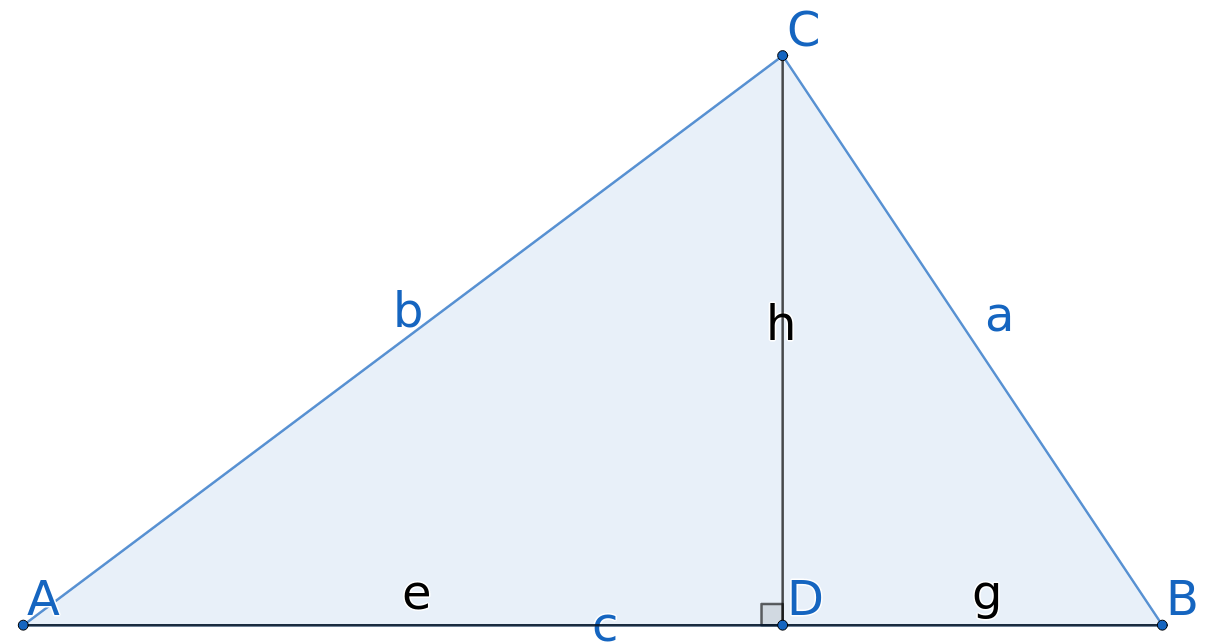
\includegraphics[width=0.5\textwidth]{triangulo.png}
\end{figure}

Considere os triângulos $\Delta CDB$ e $\Delta ACB$. Por semelhança de triângulos,
\begin{align*}
    \frac{a}{g} = \frac{c}{a} \implies a^2 = cg
\end{align*}

Considere também os triângulos $\Delta ADC$ e $\Delta ACB$. Por semelhança de triângulos,
\begin{align*}
    \frac{b}{c-g} = \frac{c}{b} \implies b^2 = c^2 - cg \implies cg = c^2 - b^2
\end{align*}

Combinando as equações, temos que
\begin{align*}
    a^2 = cg \implies a^2 = c^2 - b^2 \implies a^2 + b^2 = c^2
\end{align*}
\end{proof}


\section*{Exercício 3}

Vamos provar que $ (X \cap Y) \cup (X \cap Z) \subseteq X \cap (Y \cup Z)$:

\begin{proof}
\begin{align*}
    \alpha \in (X \cap Y) \cup (X \cap Z) &\iff (\alpha \in X \land \alpha \in Y) \lor (\alpha \in X \land \alpha \in Z) \\
    &\iff (\alpha \in X) \land (\alpha \in Y \lor \alpha \in Z) \\
    &\iff \alpha \in X \cap (Y \cup Z)
\end{align*}
\end{proof}

\section*{Exercício 8}

\begin{itemize}
    \item $\Z \cap \N = \N$
    \item $\Z \cup \N = \Z$
    \item $\set{x \in \Z : \frac{3}{2} \leq x \leq 10} \cap [6] = \set{x \in \Z : 1.5 \leq x \leq 10} \cap \set{1,2,3,4,5,6} = \set{ 2, 3, 4, 5, 6 }$
    \item $([n] \setminus [n - 3]) \cap ([n-1] \setminus [n - 4]) = \set{n-2, n-1, n} \cap \set{n-3, n-2, n-1} = \set{n-2, n-1}$
\end{itemize}

\section*{Exercício 9}
% TODO refazer exercício 9

Vamos provar que $A \cap (B \setminus C) = (A \cap B) \setminus (A \cap C)$:

\medskip

\begin{proof}
\begin{align*}
    \alpha \in (A \cap B) \setminus (A \cap C) &\iff \alpha \in (A \cap B) \land \alpha \notin (A \cap C) \\
    &\iff (\alpha \in A \land \alpha \in B) \land (\alpha \notin A \lor \alpha \notin C) \\
    *&\iff (\alpha \in A \land \alpha \in B) \land (\alpha \notin C) \\
    &\iff \alpha \in A \land (\alpha \in B \land \alpha \notin C) \\
    &\iff \alpha \in A \land (\alpha \in B \setminus C) \\
    &\iff \alpha \in A \cap (\alpha \in B \setminus C)
\end{align*}

* \textit{O $\alpha \notin A$ foi 'cancelado' pois contradiz com o $\alpha \in A$ e com a verdade da sentença completa}

Logo, os conjuntos são iguais.
\end{proof}

\end{document}